\documentclass[11pt,a4paper]{report}
\usepackage[latin1]{inputenc}
\usepackage[dutch]{babel}
\title{Algemene Handleiding Bebras:\\ Biber}

\usepackage{fullpage}
\usepackage{hyperref}
\usepackage[pdftex]{graphicx}

\setcounter{secnumdepth}{5}
\setcounter{tocdepth}{5}
\makeindex
\begin{document}
\maketitle
\parindent 0pt
\tableofcontents

% Introduction to the manual
\chapter{Inleiding}
Dit is de algemene handleiding voor de Biber versie van het Bebras platform voor Belgi"e. 

%General functions
\chapter{Algemeen}


\section{Algemene Informatie}
\subsection{Soorten gebruikers}
Er zijn vier soorten gebruikers:
\begin{itemize}
\item Een leerling kan deelnemen aan Vrije competities. Als de leerling tot een klas behoort kan hij ook klassikaal deelnemen aan de offici"ele competitie en aan lokale competities.
\item Een leerkracht is verantwoordelijk voor het samenstellen van klassen, en openen en sluiten van lokale competities voor deze klassen.
\item Een organisator is verantwoordelijk voor het maken van vragen, sets en competities.
\item Een administrator is de beheerder van de applicatie.
\end{itemize}

\subsection{Soorten Competities}
Er zijn drie types competities:
\begin{itemize}
\item Een Vrije Competitie: Deze competitie kan door alle leerlingen (volledig geregistreerd of half-geregistreerd) gespeeld worden.
\item Een Lokale Competitie: Een lokale competitie wordt aangemaakt door een leekracht voor zijn klassen, 
en kan enkel gespeeld worden door de klassen van die de leerkracht.
\item Een Offici\"ele Competitie: Deze competitie kan alleen gespeeld worden tijdens de offici\"ele Bebras week, 
ook hiervoor is een leerkracht nodig die de competitie opent voor zijn klassen.
\end{itemize}

\subsection{Levels}
Het level van een klas, en dus van alle leerlingen in die klas bepaalt welke set uit een gegeven competitie gespeeld kan worden. Een klas zal altijd de set spelen met hetzelfde level uit de competitie.
\begin{itemize}
\item Ewok: 5de en 6de leerjaar.
\item Wookie: 1ste en 2de middelbaar.
\item Padawan: 3de en 4de middelbaar.
\item Jedi: 5de en 6de middelbaar.
\end{itemize}



\section{Algemene Handelingen}

\subsection{Registreren}
Indien u nog geen account heeft zijn er een aantal mogelijkheden om een account te verkrijgen. 
\begin{itemize}
\item \textbf {Zelf registreren op webapplicatie}: Een manier om een account te verkrijgen is door u te registreren als 'half-geregistreerde' leerling.  Dit houdt in dat u een leerling-account krijgt maar (nog) niet gelinkt wordt aan een bepaalde klas of school. U kunt op deze manier meedoen aan bepaalde niet offici\"ele quizzen, en uw geschiedenis van de reeds deelgenomen quizzen bekijken. U doet dit door op de hoofdpagina op de registratie link te klikken.
\item \textbf{Via leerkracht}: Een leerling laat zich best registreren via zijn deelnemende leerkracht, en behoort zo onmiddelijk tot een klas en kan van de bijhorende voordelen genieten.
\item \textbf{Voor andere types accounts}: Een administrator registreert organisators, een organisator registreert leerkrachten. Een administrator zelf kan niet geregistreerd worden door een andere gebruiker, dus moet al op voorhand aangemaakt worden door de beheerder van de applicatie. 
\end{itemize}
Met uitzondering van leerlingen die geregistreerd worden door een leerkracht (zie sectie Leerkracht) krijgt iedereen zijn login-gegevens, bebrasId en tijdelijk paswoord, in zijn mailbox bij registratie. 

\subsection{Inloggen}
U kunt inloggen op de hoofdpagina van de applicatie. U vult uw bebrasId en uw paswoord in op de daarvoor bestemde plaats. Alle soorten gebruikers loggen in via deze methode. Na het inloggen wordt u doorverwezen naar uw persoonlijke profielpagina.
\par
Als u voor de eerste keer inlogt, wordt u verplicht na het inloggen uw toegezonden paswoord te veranderen in een paswoord naar keuze. De enige restrictie is dat het nieuwe paswoord verschillend moet zijn van het toegezonden paswoord. Daarna dient u opnieuw in te loggen, deze keer met uw eigen gekozen paswoord. Deze procedure dient alleen uitgevoerd te worden wanneer u voor de eerste keer inlogd, de andere keer zal u meteen naar uw  profielpagina doorverwezen worden. 

\subsection{Wachtwoord vergeten of veranderen?}
Op de login-pagina is er links een link beschikbaar die u leidt naar een pagina waarop u uw paswoord kunt resetten. Op die pagina moet of uw bebrasId of  uw email-adres ingevuld worden. Wanneer u een leerling bent zonder emailadres, moet aan de leerkracht gevraagd worden om uw paswoord te resetten. In alle andere gevallen wordt een mail gestuurd die een unieke link bevat die u toelaat uw paswoord te veranderen, deze link is 1 dag geldig.

\subsection{Taal selecteren en veranderen}
Doorheen de applicatie kunt u rechts boven de taal veranderen. 
De momenteel ondersteunde talen zijn: Nederlands, Frans, Duits en Engels.

\subsection{Profielpagina}
Wanneer u bent ingelogd komt u op uw persoonlijke profielpagina terecht. 
Vanaf hier kunt u verder navigeren naar de rest van de applicatie.

\subsection{Profiel aanpassen}
Via de link 'bewerk mijn gegevens' op de profielpagina kunt u uw profielgegevens aan  passen. 
Enkel de gegevens die u wilt veranderen hoeven ingevuld te worden. 

\subsection{Help pagina}
Rechts bovenaan is er een help knop. Deze brengt u op een pagina waar u een kort overzicht krijgt van hoe je aan bepaalde functionaliteiten kan geraken. 

\subsection{Handleiding downloaden}
Op de profielpagina kunt u rechts tussen de links een link vinden om deze handleiding te downloaden. Hierbij zal alleen het document worden gedownload tot het hoofdstuk van de gebruiker zelf, en niet meer de delen van de gebruikers met meer privileges.



% Manual for the pupil
\chapter{Leerling}

% A short introduction to what this user can do
\section{Introductie}
Alleen leerlingen kunnen aan wedstrijden deelnemen. Er zijn twee soorten leerlingen, leerlingen die bij een klas behoren en leerlingen die niet bij een klas horen en zich dus zelf hebben geregistreerd bij de applicatie. Alleen de leerlingen die bij een klas horen kunnen deelnemen aan de offici\"ele competitie. De andere leerlingen kunnen alleen deelnemen aan vrije competities, net zoals anonieme gebruikers maar kunnen hun geschiedenis opvragen en later eventueel hun account tot een klas laten toevoegen. Iedereen kan zich inschrijven voor een leerling account zonder klas, u hoeft hiervoor geen echte leerling te zijn.
\subsection{Profiel pagina}
Op uw profielpagina kunt u de competities zien waar u momenteel kunt aan meedoen. Ook kunt u rechts naar een link gaan om de geschiedenis van uw competities te bekijken.
\subsection{Geschiedenis bekijken}
Na het spelen van competities kunt u in uw lokale geschiedenis steeds gaan kijken hoe goed u heeft gepresteerd. Op de profielpagina vindt u link een link geschiedenis. Als u daarop klikt verschijnt er een overzicht met alle gespeelde competities.

\section{Deelnemen aan een competitie}
\subsection{Vooraf}
Om deel te nemen aan een competitie klikt u op een beschikbare competitie op de profielpagina. Daarmee komt u op het startscherm van de competitie terecht. Hier ziet u de algemene informatie over de competitie, zoals op welk level u zal deelnemen en hoeveel tijd u hebt. Hier klikt u op 'start competitie' om de competitie te starten.
\subsection{Tijdens}
Eenmaal de competitie gestart is, zult u de vragen tezien krijgen. Er zijn twee soorten vragen mogelijk:
\begin{itemize}
\item \textbf{Meerkeuze vragen}: Hier klikt u op een antwoord (A, B, C of D). U gaat na het klikken meteen naar de volgende vraag. 
\item \textbf{Open vragen}: Hier moet u een getal, woord of kleine zin invullen en daarna op bevestigen klikken.
\end{itemize}
Telkens u een antwoord hebt ingevuld zult u naar de volgende vraag gaan. Het is mogelijk om later terug te keren naar vorige vraag en ander antwoord in te vullen, dit doet u door op de lijst van vragen rechts in beeld op de gewenste vraag te klikken.
\subsection{Einde}
Als u klaar bent met de competitie klikt u op 'be\"eindig competitie'. Als u aan een lokale of vrije competitie hebt meegedaan zult u op een pagina terecht komen waarop u meteen uw resultaten kunt bekijken. U kunt per vraag ook feedback krijgen door op de feedback link van de vraag te klikken.

\begin{figure}[h!]
\centering
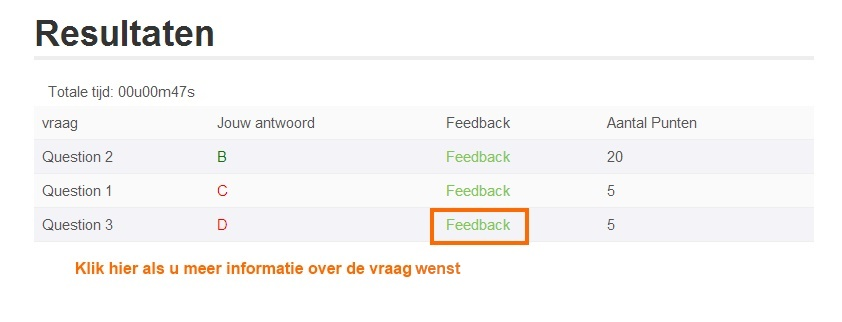
\includegraphics[width=\textwidth]{results_nl.jpg}
\caption{Scherm na het spelen van een competitie. Hier ziet u al uw antwoorden, en kunt u voor enkele vragen feedback bekijken.}
\label{fig:results}
\end{figure}

\subsection{Statistieken van een competitie bekijken}
Wanneer u naar uw geschiedenis gaat bekijken van een bepaalde competitie kunt u zien hoe het heeft gedaan in vergelijking met de anderen door op de link statistieken te klikken onder de geschiedenis van die bepaalde competitie.

\section{Offici"ele Competitie}
Deze competitie wordt jaarlijks gehouden, en verloopt zoals de andere competities, met als enige uitzondering dat na afloop u niet meteen de resultaten te zien krijgt. De leerkracht moet ook deze competitie openen voor de klas.
\begin{itemize}
  \item \textbf{Deelnemen}: U kunt enkel deelnemen aan de offici\"ele competitie als u deel bent van een klas, en deze klas aan de competitie deelneemt. Dit is de verantwoordelijkheid van de leerkracht, spoor hem aan om mee te doen indien het nog niet het geval zou zijn.
	\item \textbf{Resultaten}:  De resultaten van de offici\"ele competitie zijn pas na het aflopen van de volledige competitieduur te consulteren. De offici\"ele competitie duurt meestal een week. U kunt uw resultaten bekijken door naar uw geschiedenis te gaan of het aan uw leerkracht te vragen.
\end{itemize}


% Manual for the teacher
\chapter{Leerkracht}

%Section
\section{Introductie}
Een leerkracht registreert zichzelf door zijn persoonlijke informatie en de gegevens van alle scholen waar hij klassen wil voor aanmaken door te sturen naar een organisator. Een leerkracht is daarna verantwoordelijk voor het aanmaken van klassen behorend tot een school en het registreren van leerlingen tot deze klassen. Ook kan hij dan lokale competities maken en openen voor zijn klassen en zijn klassen laten deelnemen aan de offici\"ele competitie. 
\subsection{Profiel pagina}
Op de profielpagina kunt u uw klassen terug vinden, uw lokale competities en de offici\"ele competitie indien die op dat moment gehouden wordt.
%Sectie
\section{Competities}
Als leerkracht kunt u lokale competities maken en openstellen voor uw klas. Dit stelt u in de positie u klas te laten voorbereiden op de offici"ele competitie. 
\subsection{Lokale competitie}
\subsubsection{Aanmaken}
Als eerste dient u een lokale competitie aan te maken. Dit kan via de link 'Nieuwe Lokale Competitie' op uw profielpagina. Eerst dient uw een titel te geven, in alle talen dat u wenst, dit hoeft niet in alle talen zijn. Daarna voegt u per level maximum 1 set toe. Denk eraan dat klassen alleen maar sets kunnen spelen van hetzelfde level als hun eigen klas level. 
\subsubsection{Openen}
Na het aanmaken verschijnt de competitie op uw profielpagina, bij 'Mijn Competities'. Wanneer u daar klikt op de competitie kunt u de competitie openen voor \'e\'en of meerdere van uw klassen. Vanaf dat moment kunnen de leerlingen van deze klassen de competitie spelen.

\subsubsection{Sluiten en Resultaten bekijken}
Wanneer u de resultaten van een klas wilt downloaden moet u de competitie sluiten voor deze klas. Dit doet u door op het rood kruis naast de competitie te klikken op uw profielpagina. Hierna krijgt u de vraag voor welke van uw klassen u de competitie wil sluiten. Selecteer deze klassen en bevestig. De competitie is nu gesloten voor deze klassen, en niemand uit deze klassen kan de competitie nog spelen. Nu kunt u de resultaten downloaden voor deze klas. Dit doet u door op de klas te klikken, en zo naar de klas pagina te gaan, en daar aan de rechterkant op de link 'Zie recente competities' te klikken. Zo komt u op een pagina waar u voor deze klas alle recente competities kunt bekijken. Naast elke competitie zijn er drie download knoppen, voor elk formaat een, als u daarop klikt wordt het gewenste bestand gedownload in uw browser.

\subsubsection{Leerlingen monitoren}
Tijdens een competitie kan u uw leerlingen monitoren. Dit doet u door na het openen van een competitie op de link van de competitie te klikken op uw profielpagina. Op de volgende pagina zult u de mogelijkheid zien om de competitie te monitoren. U kunt per individuele leerling de volgende acties uitvoeren:
\begin{itemize}
	\item Extra tijd geven: Met deze knop kunt u een individuele leerling extra tijd geven om te competitie af te werken. Het formaat is uur:minuten:seconden.
	\item Verwijder geschiedenis: Met deze knop kunt u per leerling individueel de volledige geschiedenis verwijderen, en zijn deelname schrappen. Dit heeft als gevolg dat de leerling de competitie opnieuw kan doen, en geen van zijn vorige anwoorden bewaard zijn. 
	\item Heropenen competitie: Met deze knop kunt u de competitie heropenen voor een bepaalde leerling nadat hij de competitie heeft afgewerkt. Zo worden zijn huidige antwoorden behouden en kan hij verder werken of antwoorden aanpassen. Hoeveel tijd hij krijgt moet u zelf bepalen via opnieuw het formaat uur:minuten:seconden.
\end{itemize}

\begin{figure}[h!]
\centering
\includegraphics[width=\textwidth]{monitor_nl.jpg}
\caption{Scherm voor het monitoren van leerlingen tijdens competitie.}
\label{fig:monitor}
\end{figure}


\subsection{Offici\"ele competitie}
De offici\"ele competitie vindt plaats in een door de organisatie afgesproken week. Op deze week zal u op uw profielpagina onder de sectie 'Competities' de offici\"ele competitie zien staan, u zult deze herkennen door het extra sterretje. U moet deze competitie openen voor elke van uw klassen persoonlijk. U doet dit best juist voor u met uw klas aan de competitie begint. 

%Sectie
\section{Klassen en leerlingen}
\subsection{Klas toevoegen}
Een klas toevoegen kan eenvoudig via de profielpagina. Onderaan de lijst van uw klassen ziet u een groen plus symbool. Als u daarop klikt ziet u een pop-up venster verschijnen waarin u de school en het level van de klas moet selecteren en de naam van de klas kiezen. In het geval dat de school nog niet in de lijst staat, moet u een organisator contacteren met de gegevens van de nieuwe school. Zodat deze de school in het systeem kan steken.

\subsection{Klas pagina}
Als u op de naam van een klas klikt op uw profielpagina, komt u terecht op de klas pagina voor die klas. Op deze pagina staat een overzicht van alle leerlingen die op dit moment in de klas zitten. Per leerling wordt ook weergegeven of ze op dit moment online zijn. Als het bolletje voor de naam rood is, is de persoon offline, als het bolletje groen is, is de persoon online.
Een overzicht van de mogelijkheden op deze pagina:

\subsubsection{Paswoord van een leerling resetten}
Mocht \'e\'en van uw leerlingen zijn of haar paswoord vergeten zijn, kan u dit paswoord resetten. Naast elke leerling staat een reset knop, als u op deze knop klikt, ontvangt u een mail met daarin een nieuw (willekeurig en tijdelijk) paswoord voor de leerling. Die kan dan daarmee inloggen en wordt direct gevraagd een nieuw persoonlijk paswoord in te stellen.

\subsubsection{Bestaande leerling toevoegen aan klas}
Mocht u leerlingen willen toevoegen aan uw klas die al in het systeem geregistreerd zijn van vroeger bijvoorbeeld kan dat door op de groene plus knop te klikken onderaan de lijst leerlingen. In het verschenen venster moet het bebrasId van een bestaande leerling ingevuld worden. Indien dit bebrasId niet bestaat, wordt dit weergegeven, anders wordt de leerling toegevoegd aan de klas en wordt dit direct weergegeven op de klaspagina.

\subsubsection{E\'{e}n leerling toevoegen}
Vanuit de klas pagina kunt u via een link aan de linkerkant een enkele leerling toevoegen aan deze klas. Die pagina bevat een formulier waarop alle gegevens moeten ingevuld worden voor deze leerling. Alle velden behalve die van het emailadres zijn verplicht. Indien het formulier juist is ingevuld wordt de leerling geregistreerd en aan de klas toegevoegd. U ontvangt onmiddellijk een mail met daarin de logingegevens van deze nieuwe leerling. 

\subsection{Meerdere leerlingen en meerdere klassen toevoegen}
Vanop u profielpagina kunt u met een link aan de linkerkant naar de pagina gaan om meerdere leerlingen toe te voegen via het uploaden van een bestand. De pagina laat u toe nieuwe of bestaande leerlingen te registreren voor \'e\'en of meerdere klassen van een school. Toegelaten bestandsformaten zijn xls (excell 1997-2003), xlsx (excell 2007-huidige) en csv. De makkelijkste manier om aan het gevraagde formaat te voldoen, is het downloaden van een voorbeeldbestand (beschikbaar op de pagina) in een van de beschikbare formaten.
\subsubsection{Excell}
Voor zowel xls en xlsx is dit het gevraagde formaat:
De titel van elke sheet (zie figuur) bepaalt de naam van de klas. Indien de klas al bestaat in deze school -en u er verantwoordelijk voor bent-, worden de leerlingen toegevoegd aan deze klas. Indien een bestand niet voldoet aan alle richtlijnen, wordt u van de fouten op de hoogte gebracht en moet u het (gewijzigde) bestand opnieuw uploaden.
\\ \textbf{Formaat}:
\begin{itemize}
\item Rij 1: Beginjaar van het schooljaar. Dus voor schooljaar 2002-2003 is dit 2002.
\item Rij 2: Het niveau van de klas. Keuze uit: EWOK, WOOKIE, PADAWAN of JEDI.
\item Rij 3: Niets verplicht. Voor de duidelijkheid is het makkelijk om hier de kolomnamen in te vullen: (volgorde verplicht): Voornaam, Familienaam, Emailadres (optioneel), Geslacht, Taal, Geboortedatum (dd/mm/jjjj). Als laatste kan daarnaast ook nog een bebrasID ingevuld worden indien u een bestaande leerling ook wil toevoegen aan deze klas. Wanneer u het voorbeeld download zullen deze velden automatisch ingevuld worden.
\item Vanaf rij 4 worden per rij dus de gegevens van een leerling ingevuld.
\end{itemize}
\subsubsection{Csv}
Invullen verloopt analoog aan het invullen van de excell bestanden. In plaats van een nieuwe sheet te gebruiken voor elke nieuwe klas, volstaat het in dit formaat om een regel wit te laten. Voor een exact voorbeeld kunt u het voorbeeldbestand downloaden.
\subsubsection{Afhandeling}
Indien er bij het uploaden geen fouten vastgesteld worden, krijgt u daarna een mail met daarin een bestand met dezelfde extensie als bijlage. In dit bestand staan de gegevens van alle net geregistreerde leerlingen, met daarbij nu de logingegevens voor elke leerling. Indien de leerling al bestond (en dit correct ingevuld was in de BebrasID-kolom) blijft zijn paswoord hetzelfde en wordt dit niet getoond in het bestand. 
De nieuwe of ge\"updatete klassen zijn hierna ook zichtbaar op uw profielpagina.
\begin{figure}[h!]
\centering
\includegraphics[width=\textwidth]{uploadPupils_nl.jpg}
\caption{Voorbeeld van excell bestand om leerlingen te registreren.}
\label{fig:uploadPupils}
\end{figure}

\subsection{Downloaden klassen van school}
Via de 'download klassen' link op de profielpagina komt u op een pagina waar u de mogelijkheid heeft om alle klassen van uw huidige school te downloaden in een gewenst formaat (excell xlsx, excell xls, csv). U kunt kiezen of u de klassen die dit jaar geregistreerd zijn wil downloaden, of de klassen die vorig jaar geregistreerd waren. Dit kan een handig hulpmiddel zijn wanneer u aan het begin van een schooljaar leerlingen wil registreren die eerder al aan de competitie hebben meegedaan, en nog steeds op dezelfde school zitten.

\subsection{Leerlingen samenvoegen}
Wanneer u op de link 'Samenvoegen van Leerlingen' klikt op de profiel pagina kunt u profielen van leerlingen uit uw scholen die zich per ongeluk twee keer hebben geregistreerd samenvoegen. Hiervoor vult u de naam in van de persoon die twee of meerdere accounts heeft. Wanneer u op zoeken klikt krijgt u een overzicht terug van alle mogelijke bebrasIds die onder deze naam zijn aangemaakt. Selecteer eerst alle accounts van die persoon, dit doet u door gewoon op de gewenste bebrasId te klikken. Elk geselecteert account komt in de lijst eronder terecht, daarvan kiest u 1 account dat nog dient over te blijven. Dan klikt u op bevestigen en zullen de accounts die in de lijst staan maar niet het account zijn dat u hebt gekozen verwijderd worden, en zal de geschiedenis van al deze leerlingen samengevoegd worden naar het ene geselecteerde account.

\subsection{Statistieken downloaden van leerlingen}
U kunt op verschillende manieren statistieken van uw leerlingen bekijken. Ten eerste kunt u individuele statsitieken zien tijdens het monitoren van leerlingen. Ten tweede kunt u na het sluiten van de competitie statistieken downloaden op de klas pagina zelf. 

% Manual for the organiser
\chapter{Organisator}

%Sectie
\section{Introductie}
Een organisator heeft vooral taken die de organisatie van de applicatie betrekken. Hij is verantwoordelijk voor het registreren van leerkrachten en scholen. Hij heeft de zeer belangrijke taak het schooljaar te be"eindigen tussen twee schooljaren door. Ook is hij de enige gebruiker die vragen kan uploaden en unrestricted competities kan aanmaken.  Hij is ook de enige die een offici\"ele competitie kan samenstellen, aanmaken, openen en sluiten.


%Sectie
\section{Scholen en Leerkrachten}
Een organisator maakt leerkrachten en hun desbetreffende scholen aan. Eens een leerkracht en zijn school in het systeem zitten kan de leerkracht zelf klassen aanmaken en leerlingen aan deze klassen toevoegen. 
\subsection{Leerkracht en School Registreren}
Wanneer u een leraar wil registreren hebt u zijn persoonlijke gegevens nodig, en de gegevens van alle scholen waarin hij klassen heeft waarmee hij wil deelnemen aan de competities. Deze gegevens worden best bekomen via e-mail. Eens u deze gegevens hebt is het nodig om de kijken of de school/scholen al in het systeem zitten. Als dit niet het geval is dient u deze te registreren via de link 'registreer school' op de profielpagina. Hier vult u alle gegevens in van de school, en die komt dan meteen in het systeem.
Daarna kunt u de leerkracht registreren in het systeem, dit doet u via de link 'registreer leerkracht' op de profielpagina. Op de volgende pagina vult u alle velden in en selecteert u zijn scholen uit de lijst van scholen die al in het systeem zitten. 
Na registratie krijgt de leraar per e-mail zijn inloggegevens.

\subsection{Account leerkracht overnemen}
Het tijdelijk overnemen van de account van een leerkracht kan eenvoudig door na het inloggen, rechts boven op de knop 'Mimick User' te klikken. Er zal een pop-up venster verschijnen waarin u de bebrasId invult van de leerkracht waarvan u de account tijdelijk wil uitvoeren. Wanneer u een juiste bebrasId invult zal u meteen worden doorgestuurd naar de profielpagina van de desbetreffende leerkracht. Vanaf nu kunt u alle functies uitvoeren die die leerkracht kan. Wanneer u gedaan bent klikt u op de 'uitloggen' knop rechts boven en komt u terug naar uw eigen profielpagina.

\subsection{Een schooljaar be\"eindigen}
Op het einde van het schooljaar is het noodzakelijk dat een organisator de huidige klassen desactiveert. Hij doet dit door op zijn profielpagina naar de link 'be"eindig schooljaar te gaan, de instructies te lezen en op "be"eindig" te klikken. Dit zorgt ervoor dat alle leerlingen en leerkrachten hun klas verliezen. Dit wordt best gedaan tussen 1 juli en 31 augustus. Deze handeling kan niet ongedaan gemaakt worden, wees hier dus voorzicht mee.

%Sectie
\section{Vragen, Sets en Competities}
Organisatoren zijn verantwoordelijk voor het uploaden van vragen naar de applicatie, het selecteren van deze vragen op basis van hun moeilijkheid om een set te maken, en op basis van sets een competitie te maken met verschillende sets voor verschillende leeftijdscategorie"en. 

\subsection{Aanmaken of aanpassen van vragen}
U heeft twee mogelijkheden om vragen aan te maken of te verwijderen. De eerste methode bestaat erin een zip file up te loaden naar de applicatie met de vragen en feedback in html formaat. De tweede methode bestaat erin de ingebouwde 'what you see is what you get' html editor te gebruiken. 

\subsubsection{Uploaden van zip bestand}
Voor deze methode moet u voor al uw vragen de vragen (html formaat)/feedback (html formaat)/afbeeldingen bundelen in een zip bestand en dit bestand uploaden naar de applicatie. Wanneer dit geslaagd zult u naar de volgende pagina gaan en moet u beslissen of u een huidige vraag in de databank wil aanpassen of een nieuwe vraag wil toevoegen. Daarna moet u beslissen voor in welke taal de vraag geschreven is. Wanneer dit gebeurd is moet u de juiste vragen selecteren, zowel voor de vraag als eventueel voor de feedback. U moet ook telkens een antwoord meegeven. U heeft de keuze uit een meerkeuze antwoord (A, B, C of D), of een reguliere expressie wat inhoudt dat u eender welke woord, zin of getallen kan invullen. Als u klaar bent kunt u bevestigen om de vraag in de databank te plaatsen of aan te passen.
\subsubsection{Met wysiwyg editor}
Deze methode is gelijkend aan de methode hierboven. Hiervoor dient u alleen geen bestanden te uploaden. U typt gewoon de vraag in een word achtige editor. In plaats van bestanden te selecteren voor uw vraag en uw feedback dient u de geschikte editor te gebruiken voor zowel de vraag als de feedback. Deze staan onderaan de pagina. 
\begin{figure}[h!]
\centering
\includegraphics[width=\textwidth]{uploadQuestion_nl.jpg}
\caption{Scherm voor het uploaden of aanpassen van vragen.}
\label{fig:uploadQuestion}
\end{figure}


\subsection{Een vragenset aanmaken}
Om de vragen te bundelen tot een set moet u het volgende doen. U drukt op de 'cre"eer vragen set' link, deze kunt u vinden op uw profielpagina of op de 'beheer vragen pagina'. U moet op dit scherm twee dingen doen. Ten eerste moet u de vragen selecteren en ten tweede moet u de algemene informatie over de set invullen. 

\begin{itemize}
\item \textbf{Algemene informatie}: Bovenaan de pagina kunt u drukken op 'info kiezen' om de tekstveldjes te tonen waar u de \textbf{titel} in verschillende talen kunt opgeven. Ook dienen de volgende dingen ingevuld te worden. De \textbf{tijdslimiet} in minuten. Het \textbf{publiek} van de set bepaalt voor welke competities deze set kan gebruikt worden, officie\"el kan alleen gebruikt worden voor de offici\"ele competitie, lokaal alleen door leerkrachten voor lokale competities op te stellen. Wanneer het publiek op onbeperkt wordt gezet, wordt een vrije competitie aangemaakt met die ene set, zolang de set zichtbaar is. De \textbf{zichtbaarheid} bepaalt of de set door andere gebruikers dan organisatoren gezien kan worden en of de set al gebruikt kan worden om competities aan te maken. En als laatste het \textbf{niveau} (Ewok, Wookie, Padawan, Jedi), dit bepaalt welke klassen deze set kunnen spelen, want alleen klassen met hetzelfde level kunnen een set van een bepaald level spelen.

\item \textbf{Vragen selecteren}: U ziet een lijst met alle beschikbare vragen, tussen haakjes staat steeds in welke talen de vraag allemaal beschikbaar is. Om een vraag toe te voegen aan de vragenset drukt u op de checkbox voor de vraag. Als u op deze checkbox drukt verschijnen er drie input velden. E\'en om de moeilijkheidsgraad van deze vraag voor deze set te selecteren, \'e\'en voor het aantal punten dat de vraag oplevert bij een juist antwoord, en \'e\'en voor het aantal punten dat worden afgetrokken bij een slecht antwoord. Deze beide getallen moeten positief zijn. 
\end{itemize}
Rechts vindt u een lijst van alle geselecteerde vragen. Wenst u de vragenset op te slaan, dan drukt u op de 'cre"eren' knop.

\begin{figure}[h!]
\centering
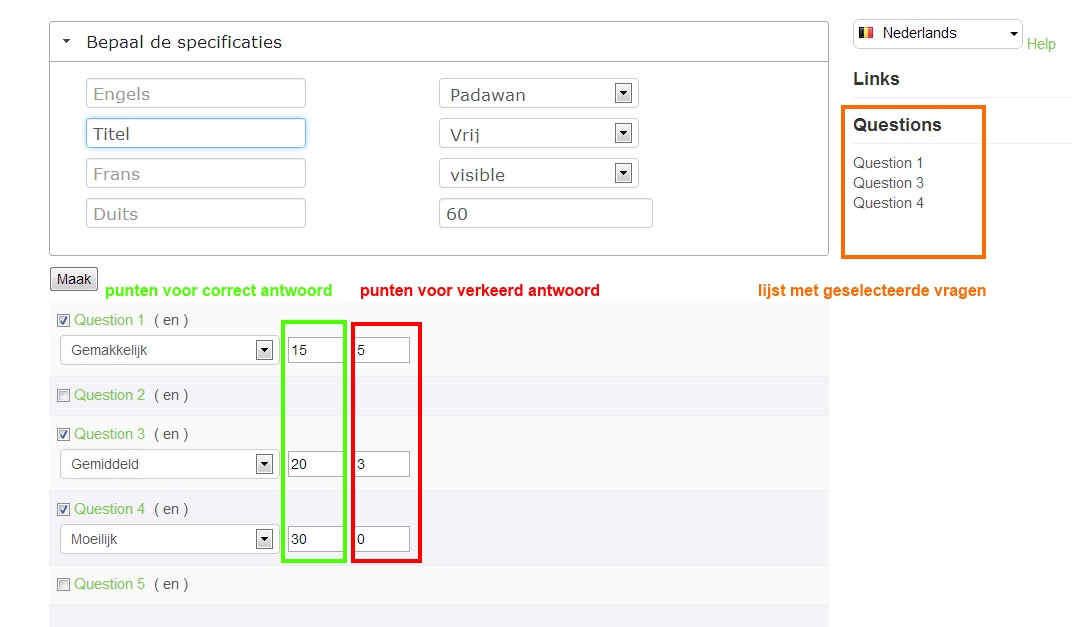
\includegraphics[width=\textwidth]{makesets_nl.jpg}
\caption{Scherm voor het aanmaken van vragensets, met verduidelijking waar wat staat en waar u wat moet invullen.}
\label{fig:makesets}
\end{figure}

\subsection{Vragensets beheren}
Op deze pagina kunt u sets verwijderen, aanpassen, en van zichtbaarheid veranderen.
Om de zichtbaarheid te veranderen kunt u op de groene pijlen klikken naast een set, deze zullen de zichtbaarheid van een set verlagen (pijl omlaag) of verhogen (pijl omhoog). Als u op het rood kruist klikt naast een set zult u deze set verwijderen. Wilt u een set aanpassen dan klikt u op het potlood naast de set, en komt u op een scherm terecht dat hetzelfde is als het scherm voor het maken van vragensets. De enige verandering nu is dat alle gegevens al zijn ingevuld, en u deze kunt aanpassen waar nodig.

\subsection{Een competitie aanmaken}
\textbf{Vrije Competitie}: Een vrije competitie wordt automatisch aangemaakt wanneer u een vragenset aanmaakt van het type 'vrij' die open is gesteld. 
\\ \\
\textbf{Offici\"ele Competitie}: Deze wordt aangemaakt op de volgende manier. 
U klikt hiervoor op de link 'maak nieuwe competitie' rechts op de profielpagina. U dient twee zaken te doen.
\begin{itemize}
		\item \textbf{Naam geven}: U vult in elke taal dat u wilt een titel in. 
		\item \textbf{Sets selecteren}: Voor elk level kiest u ten hoogste 1 set. Alle sets van het type 'Offici\"eel' zullen in de lijst verschijnen. 
\end{itemize}

\subsection{Competities Openen}
Op uw profielpagina ziet u de lijst van offici\"ele competities die u hebt aangemaakt. Het slotje naast elke competitie toont of de competitie geopend of gesloten is. U kunt een competitie openen/sluiten door op het slotje te klikken, of door op de competitie te klikken, en te bevestigen.

\subsection{Statistieken}
U kunt per set statistieken bekijken op de 'beheer sets' pagina, door naast de gewenste competitie op de statistieken knop te klikken.


% Manual for the admin
\chapter{Admin}
\section{Introductie}
Een administrator account wordt aangemaakt door de applicatiebeheerder. De voornaamste taak die een administrator heeft is het registreren van organisatoren en het beheren van de ftp servers.
\section{Organisator registreren}
Via de link 'Registreer organisator' in de links op de profielpagina komt u op de registratiepagina. Deze pagina toont een formulier met de nodige velden om een nieuwe organisator te registreren. Alle velden zijn verplicht.
Na registratie krijgt de organisator per email zijn inloggegevens.

\section{Account organisator/leerkracht overnemen}
Een administrator kan het account overnemen van een organisator of van een leerkracht. Hij doet dit op dezelfde manier als dat een organisator het account van een leerkracht overneemt. Hij klikt hiervoor rechtsboven op de profielpagina op 'Mimick User', en vult dan in het pop-up scherm de bebrasId van de organisator/leerkracht in die hij wil overnemen.

\section{Beheren van FTP-servers}
ALs u op de link 'beheer ftp-servers' klikt op uw profielpagina komt u terecht op de pagina waar u een overzicht ziet van de huidige ftp-servers. Op deze pagina kunt u servers toevoegen, verwijderen en editeren. 
\begin{itemize} 
	\item Server toevoegen: Klik op de knop rechts onder. U krijgt een pagina te zien waarop u alle nodige gegevens dient in te vullen. 
	\item Server aanpassen: Klik in het overzicht op het potlood rechts naast de server die u wilt aanpassen. U zult op een pagina komen waarop u alle gegevens kunt aanpassen.
	\item Server verwijderen: Klik in het overzicht op het verwijder icoon rechts naast de server die u wilt verwijderd, de server wordt meteen verwijderd uit het systeem.
\end{itemize}

\begin{figure}[h!]
\centering
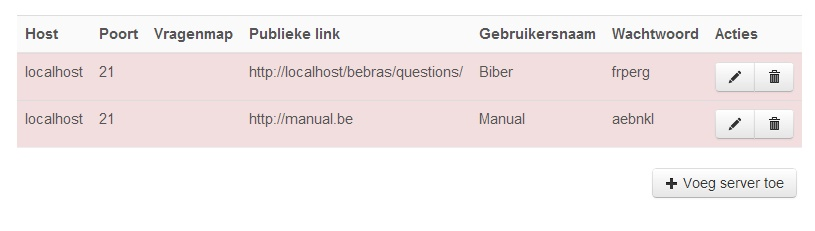
\includegraphics[width=\textwidth]{manageftp_nl.jpg}
\caption{Scherm voor het beheren van ftp servers: hier kunt u servers toevoegen, verwijderen, aanpassen en de gegevens ervan bekijken.}
\label{fig:manageftp}
\end{figure}


\end{document}